304. \begin{figure}[ht!]
\center{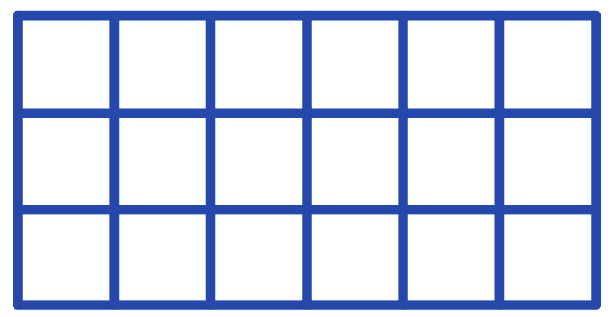
\includegraphics[scale=0.35]{tab.png}}
\end{figure}\\
Расставьте в каждую клетку таблицы $3\times6$ букву К, А или С так, чтобы у каждой К было 4 соседа А, а у каждой С было ровно два соседа А, а у каждой А среди соседей есть и К, и С. Соседи считаются только по стороне.\\
